%
% koordinaten.tex
%
% (c) 2018 Prof Dr Andreas Müller, Hochschule Rapperswil
%
\section{Koordinaten%
\label{skript:koordinaten}}
\rhead{Koordinaten}
In diesem Abschnitt schlagen wir die Brücke zwischen der Algebra der
Vektoren und der Geometrie.
Dabei wir müssen natürlich gewisse Annahmen darüber machen, was
wir von der Geometrie benutzen wollen.
Wir achten darauf, möglichst einfache Voraussetzungen zu machen,
zum Beispiel möchten wir nicht voraussetzen, dass wir bereits
die Länge einer Strecke messen können (auf das dazu notwendige
Skalarprodukte gehen wir in Kapitel~\ref{chapter:orthogonalitaet} ein).
Wir brauchen aber mindestens den Begriff von Punkt, Gerade und Strecke
sowie die Parallelenkonstruktion.
Dies können wir in den folgenden Axiomen zusammenfassen:
\begin{compactenum}
\item
Zu zwei Punkten kann man immer eine Gerade durch die beiden Punkte
finden.
\item
Zu einer Gerade in der Ebene und einem Punkt nicht auf der Geraden
gibt es immer eine Gerade durch den Punkt, die die erste Gerade nicht
schneidet.
\item
Zu drei Punkten im Raum, die nicht auf einer Geraden liegen, gibt es
eine Ebene, die die drei Punkte enthält.
\item
Zu einer Ebene im Raum und einem Punkt nicht in der Ebene gibt es eine
zweite Ebene durch den Punkt, die die erste Ebene nicht schneidet.
\end{compactenum}
Aus den ersten zwei Punkten lässt sich zum Beispiel ableiten, dass
man zu drei Punkten immer ein Parallelogramm konstruieren kann.
Diese Konstruktion ist in Abbildung \ref{skript:affin:parallelogramm}
dargestellt.
Mit ihr kann man zwei Strecken vergleichen, ohne ihre Länge messen
zu müssen.
Wenn die beiden Strecken Seiten eines Parallelogramms sind, dann
sind sie gleich.
Man kann damit Strecken auch mehrfach aneinander hängen, was einer
Multiplikation mit einer natürliche Zahl entspricht.
\begin{figure}
\centering
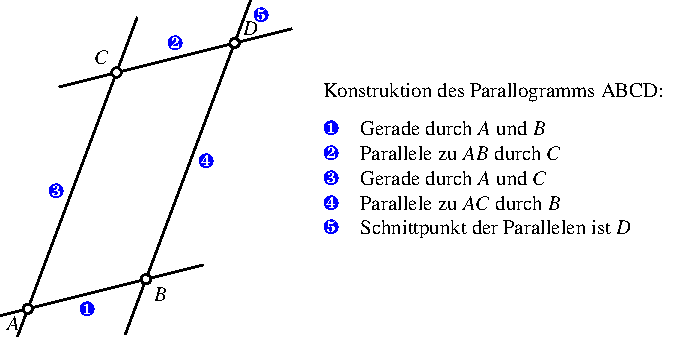
\includegraphics{3/images/parallelogramm.pdf}
\caption{Parallelogramm-Konstruktion. Konstruiere zu drei Punkten
$A$, $B$ und $C$ die vierte Ecke $D$ eines Parallelogramms.
\label{skript:affin:parallelogramm}}
\end{figure}

Mit der Strahlensatz-Konstruktion in
Abbildung~\ref{skript:affin:strahlensatz}
kann man eine Strecke in einem beliebigen rationalen Verhältnis aufteilen.
Man kann also eine Strecke mit einer rationalen Zahl ``multiplizieren''
ohne dass m an ihre Länge messen kann.
\begin{figure}
\centering
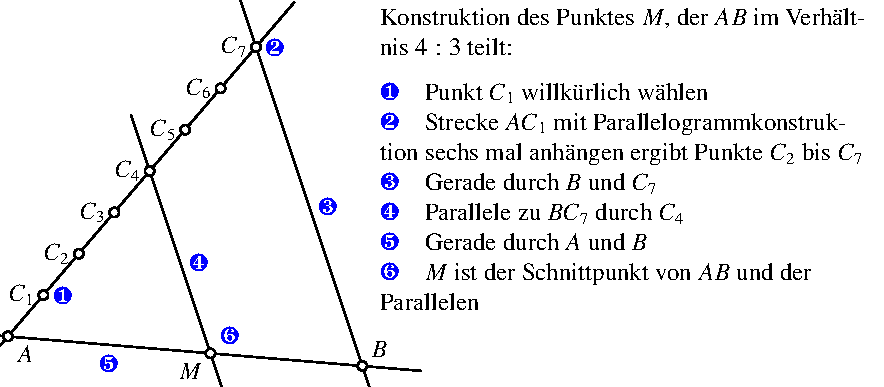
\includegraphics{3/images/strahlensatz.pdf}
\caption{Strahlensatz-Konstruktion. 
Teile eine gegebene Strecke in einem rationalen Verhältnis, hier wird
die Strecke $AB$ im Verhältnis $4:3$ geteilt.
\label{skript:affin:strahlensatz}}
\end{figure}

Man beachte aber, dass es damit noch nicht möglich ist, zwei Strecken
zu vergleichen, die nicht parallel sind.
Dazu müsste man eine Strecke drehen können, so wie man das zum Beispiel
mit einem Zirkel machen kann.
Die Geometrie, die wir hier entwickeln, verwendet aber keinen Zirkel,
sondern nur Geraden, Punkte und Parallelität.
Sie enthält also wesentlich weniger, als die euklidische Geometrie, die
man in der Sek lernt.
Sie heisst die {\em affine Geometrie}.
\index{affine Geometrie}

%
% Punkte und Vektoren
%
\subsection{Punkte und Vektoren}
Die Geometrie macht Aussagen über Punkte in der Ebene und im Raum.
Kein Punkt spielt eine besondere Rolle, alle Punkte sind gleichberechtigt.
Die Algebra der Vektoren kennt dagegen einen ausgezeichneten Vektor,
nämlich den Nullvektor, und sie kennt Operationen, die kein offensichtliches
Gegenstück in der Geometrie haben, die Multiplikation mit Zahlen und
die Addition von Vektoren.
Es braucht daher eine Übersetzung, welche Punkte auf Vektoren
abbildet und den algebraischen Operationen einen geometrischen
Sinn gibt.

\subsubsection{Nullpunkt und Ortsvektoren}
Wenn es eine Abbildung von Punkten auf Vektoren gibt, dann muss dem
Nullvektor ein ausgezeichneter Punkt entsprechen, den wir meist mit 
$O$ bezeichnen und {\em Nullpunkt} oder {\em Ursprung} nennen.
Der Buchstabe $O$ kommt vom lateinischen Wort {\it origo}, welches
Ursprung bedeutet.

Einem Punkt $P$ der Ebene können wir jetzt einen Pfeil
von $O$ nach $P$ zuordnen.
\index{Pfeil}
Einen Pfeil kann man in der Ebene parallel verschieben,
wie zum Beispiel die Parallelogramm-Konstruktion zeigt.
Alle parallelen Pfeile sind gleichwertig, wir bezeichnen
jeden dieser Pfeile als Vektor $\overrightarrow{OP}$, den
wir auch den {\em Ortsvektor} des Punktes $P$ nennen
(Abbildung~\ref{skript:affin:ortsvektor}).
\index{Ortsvektor}
\begin{figure}
\centering
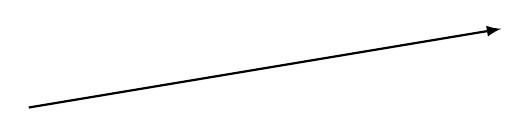
\begin{tikzpicture}[>=latex,thick]
\coordinate (O) at (0,0);
\coordinate (P) at (6,1);
\draw[->] (O)--(P);
\end{tikzpicture}
\caption{
Ursprung $O$ und Ortsvektor $\protect\overrightarrow{OP}$ des Punktes $P$
\label{skript:affin:ortsvektor}
}
\end{figure}

\begin{konvention}
Den Ortsvektor des Punktes $P$ bezeichnen wir üblicherweise mit dem 
zugehörigen Kleinbuchstaben $\vec{p}$, also
\[
\overrightarrow{OP} = \vec{p}.
\]
\end{konvention}

\subsubsection{Algebraische Operationen}
Wir müssen jetzt die algebraischen Operationen für Vektoren,
die wir für die lineare Algebra brauchen, für Ortsvektoren erklären:
\begin{enumerate}
\item
Addition: Pfeile werden mit Hilfe der Parallelogramm-Konstruktion
von Abbildung~\ref{skript:affin:parallelogramm}
aneinander gehängt:
\begin{center}
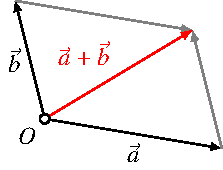
\includegraphics{3/images/addition.pdf}
\end{center}
\item
Multiplikation mit einer Zahl: Um einen Vektor mit der rationalen
Zahle zu multiplizieren, wird die Strahlensatz-Konstruktion
von Abbildung~\ref{skript:affin:strahlensatz} gewählt.
\end{enumerate}
Aus den Konstruktionen folgt, dass die Eigenschaften der Rechenoperationen
mit Vektoren genau den Eigenschaften der geometrischen Operationen
mit Pfeilen entsprechen.

%
% Basis und Koordinatensysteme
%
\subsection{Basis und Koordinatensystem}
Ein Koordinatensystem ermöglicht, jeden beliebigen Punkt des Raumes mit
Hilfe weniger Zahlen zu beschreiben.
Der ausgezeichnete Punkt $O$ reicht dafür noch nicht. 
Ein Koordinatensystem erhalten wir erst, wenn zusätzlich eine Menge
$\mathcal{B}=\{\vec{b}_1,\dots,\vec{b}_n\}$ von Vektoren vorgegeben ist.
Wir sagen, der Punkt $P$ hat die Koordinaten $(x_1,\dots,x_n)$, wenn 
gilt
\[
\vec{p}=\operatorname{OP} = x_1\vec{b}_1+\dots+x_n\vec{b}_n.
\]
Meist geht man intuitiv davon aus, dass die Vektoren von $\mathcal{B}$
aufeinander senkrecht stehen und Länge $1$ haben, diese Bedingung
ist aber unnötig, ja im Moment haben wir noch nicht einmal die
nötigen Hilfsmittel, um Länge und Zwischenwinkel zu berechnen, diese
werden erst im Kapitel~\ref{chapter:orthogonalitaet} bereitgestellt.

Nicht jede Menge $\mathcal{B}$ von Vektoren ist gleichermassen
zur Konstruktion eines Koordinatensystems geeignet.
Zu einem Punkt sollte es genau einen Satz von Koordinaten geben,
die diesen Punkt beschreiben.
Gäbe es zwei Koordinaten $(x_1,\dots,x_n)$ und $(x_1',\dots,x_n')$,
die auf den selben Ortsvektor $\vec{p}$ abgebildet werden, dann müsste gelten
\[
\vec{p}=
x_1\vec{b}_1+\dots+x_n\vec{b}_n
=
x_1'\vec{b}_1+\dots+x_n'\vec{b}_n.
\]
Bringt man alles auf eine Seite, erhält man die Gleichung
\[
(x_1-x_1')\vec{b_1}
+\dots+
(x_n-x_n')\vec{b_n}
=0.
\]
Dies ist ein homogenes lineares Gleichungssystem, und wir möchten, dass
es nur eine Lösung hat.
Nach Abschnitt~\ref{skript:section:linabh} ist dies genau dann der Fall,
wenn die Vektoren $\vec{b}_1,\dots,\vec{b}_n$ linear unabhängig sind.

\begin{definition}
Eine Menge $\mathcal{B}=\{\vec{b}_1,\dots,\vec{b}_n\}$ heisst eine Basis,
wenn die Vektoren linear unabhängig sind und sich damit alle Ortsvektoren
ausdrücken lassen.
\end{definition}

Es ist aus der Parallelgramm-Konstruktion klar, dass in der Ebene zwei 
Basisvektoren genügen, während für den dreidmensionalen Raum drei
Basisvektoren nötig sind.
\begin{figure}
\centering
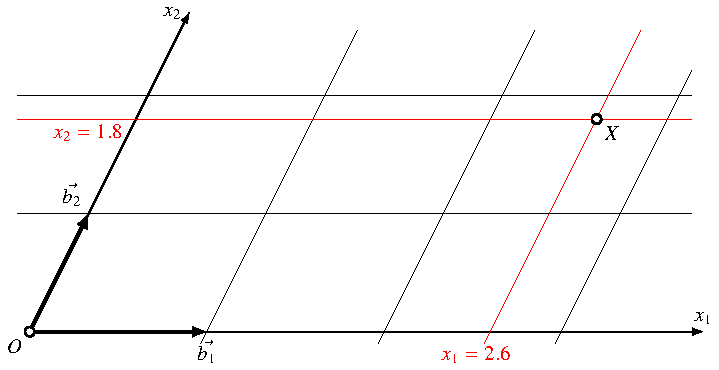
\includegraphics{3/images/coord2d.pdf}
\caption{Koordinaten $(x_1,x_2)$ des Punktes $X$ in dem durch die
Basis  $\mathcal{B}=\{\vec{b}_1,\vec{b}_2\}$ definierten Koordinatensystem.
\label{skript:affin:coord2d}}
\end{figure}
In Abbildung~\ref{skript:affin:coord2d} ist die Darstellung eines Punktes
$X$ in der Basis $\mathcal{B}=\{\vec{b}_1,\vec{b}_2\}$ dargestellt.
\begin{figure}
\centering
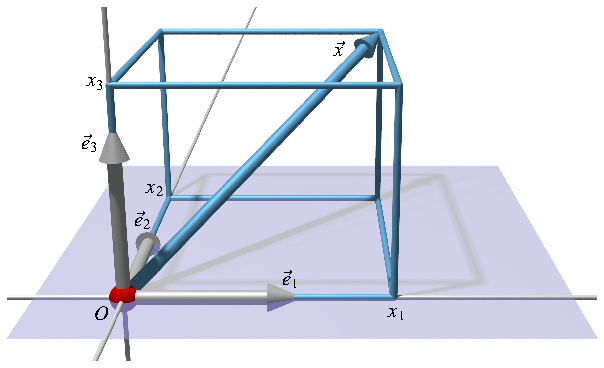
\includegraphics{3/images/coordsystem.pdf}
\caption{Koordinaten $(x_1,x_2,x_3)$ des Punktes $X$ mit Ortsvektor $\vec{x}$
in der Basis $\mathcal{B}=\{\vec{e}_1,\vec{e}_2,\vec{e}_3\}$.
\label{skript:affin:coordsystem}}
\end{figure}
In Abbildung~\ref{skript:affin:coordsystem} ist die Darstellung eines Punktes
$X$ mit Ortsvektor $\vec{x}$ in der Basis
$\mathcal{B}=\{\vec{e}_1,\vec{e}_2,\vec{e}_3\}$
gezeigt.
Hier werden spezielle Basisvektoren verwendet, die orthogonal sind und Länge
$1$ haben.

Sobald eine Basis festgelegt ist, können wir beliebige Vektoren in dieser
Basis ausdrücken. 
Wir verwenden wieder die Spaltenschreibweise dafür.
Der Ortsvektor des Punktes $X$ mit den Koordinaten $(x_1,x_2,x_3)$ ist dann
\[
\overrightarrow{OX}
=
\vec{x}
= 
\begin{pmatrix}x_1\\x_2\\x_3\end{pmatrix}.
\]
Die algebraischen Rechenoperationen stimmen genau mit den geometrischen
Konstruktionen überein.
Man beachte, dass die Basisvektoren selbst die Koordinaten
\[
\begin{aligned}
\vec{b}_1 &= \begin{pmatrix}1\\0\\0\end{pmatrix}, &
\vec{b}_2 &= \begin{pmatrix}0\\1\\0\end{pmatrix} &
          &\text{und}&
\vec{b}_3 &= \begin{pmatrix}0\\0\\1\end{pmatrix}
\end{aligned}
\]
haben.

%
% Linearkombination
%
\subsection{Linearkombination und aufgespannter Raum}
Seien jetzt drei Vektoren $\vec{a}_1$, $\vec{a}_2$ und $\vec{a}_3$ gegeben.

\subsubsection{Linearkombination}
wir möchten verstehen, wie eine Linearkombination
\[
\vec{y}
=
\xi_1\vec{a}_1
+
\xi_2\vec{a}_2
+
\xi_3\vec{a}_3
\]
berechnet wird.
Wir gehen davon aus, dass eine Basis gewählt worden ist, und dass
folglich die Vektoren $\vec{a}_i$ als Spaltenvektoren geschrieben
werden können, die wir
\[
\begin{aligned}
\vec{a}_1 &= \begin{pmatrix}a_{11}\\a_{21}\\a_{31}\end{pmatrix}, &
\vec{a}_2 &= \begin{pmatrix}a_{12}\\a_{22}\\a_{32}\end{pmatrix}
&&\text{und}&
\vec{a}_3 &= \begin{pmatrix}a_{13}\\a_{23}\\a_{33}\end{pmatrix}
\end{aligned}
\]
schreiben.

Die Linearkombination hat dann die Komponenten
\[
\vec{y}
=
\begin{pmatrix}a_{11}\\a_{21}\\a_{31}\end{pmatrix}
\xi_1
+
\begin{pmatrix}a_{12}\\a_{22}\\a_{32}\end{pmatrix}
\xi_2
+
\begin{pmatrix}a_{13}\\a_{23}\\a_{33}\end{pmatrix}
\xi_3
=
\begin{pmatrix}
a_{11}\xi_1+a_{12}\xi_2+a_{13}\xi_3\\
a_{21}\xi_1+a_{22}\xi_2+a_{23}\xi_3\\
a_{31}\xi_1+a_{32}\xi_2+a_{33}\xi_3
\end{pmatrix}
=
\underbrace{
\begin{pmatrix}
a_{11}&a_{12}&a_{13}\\
a_{21}&a_{22}&a_{23}\\
a_{31}&a_{32}&a_{33}
\end{pmatrix}}_{\displaystyle=A}
\underbrace{
\begin{pmatrix}
\xi_1\\\xi_2\\\xi_3
\end{pmatrix}}_{\displaystyle=\vec{\xi}}
=
A\vec{\xi}
\]
Die Bedeutung des Produktes Matrix mal Vektor ist also die Linearkombination
der Spaltenvektoren der Matrix mit den Koeffizienten des Spaltenvektors.

\subsubsection{Aufgespannter Raum und Bildraum}
Die Vektoren $\mathcal{A}=\{\vec{a}_1,\dots,\vec{a}_l\}$ müssen nicht
unbedingt eine Basis bilden.
Es ist also durchaus möglich, dass die Menge aller Linearkombinationen
nur eine Telmenge des Raums aller Vektoren ausmacht.
Man nennt
\[
\langle
\mathcal{A}
\rangle
=
\langle
\vec{a}_1,\dots,\vec{a}_n
\rangle
=
\{
\xi_1\vec{a}_1+\dots+\xi_n\vec{a}_n\;|\; \xi_i\in\mathbb R
\}
\]
den von den Vektoren in $\mathcal{A}$ {\em aufgespannten Raum}.
\index{aufgespannter Raum}
Da $\langle\mathcal{A}\rangle$ auch die Menge aller Vektoren der
Form $A\vec{\xi}$ ist, heisst $\langle\mathcal{A}\rangle$
auch der {\em Bildraum} $\operatorname{im}A$ der Matrix $A$.
\index{Bildraum}

\begin{beispiel}
Die Vektoren \[
\mathcal{A}=\left\{
\begin{pmatrix}1\\2\\3\end{pmatrix},
\begin{pmatrix}3\\2\\1\end{pmatrix}
\right\}
\]
spannen einen zweidimensionalen Unterraum von $\mathbb R^3$ auf.
Man finde
die Koordinaten des Vektors
\[
\vec{v}
=
\begin{pmatrix}
0\\4\\8
\end{pmatrix}
\]
als Linearkombination der Vektoren von $\mathcal{A}$.

Dazu muss man das Gleichungssystem $\vec{v}=A\vec{\xi}$ lösen:
\[
\begin{tabular}{|>{$}c<{$}>{$}c<{$}|>{$}c<{$}|}
\hline
\xi_1&\xi_2&\\
\hline
1%
\begin{picture}(0,0)
\color{red}\put(-3,4){\circle{12}}
\end{picture}%
&3&0\\
2&2&4\\
3%
\begin{picture}(0,0)
\color{blue}\drawline(-8,-2)(-8,25)(2,25)(2,-2)
\end{picture}%
&1&8\\
\hline
\end{tabular}
\rightarrow
\begin{tabular}{|>{$}c<{$}>{$}c<{$}|>{$}c<{$}|}
\hline
\xi_1&\xi_2&\\
\hline
1&3&0\\
0&-4%
\begin{picture}(0,0)
\color{red}\put(-7,4){\circle{15}}
\end{picture}%
&4\\
0&-8%
\begin{picture}(0,0)
\color{blue}\drawline(-15,-2)(-15,10)(1,10)(1,-2)
\end{picture}%
&8\\
\hline
\end{tabular}
\rightarrow
\begin{tabular}{|>{$}c<{$}>{$}c<{$}|>{$}c<{$}|}
\hline
\xi_1&\xi_2&\\
\hline
1&3%
\begin{picture}(0,0)
\color{blue}\drawline(-8,10)(-8,-2)(1,-2)(1,10)
\end{picture}%
&0\\
0&1&-1\\
\hdashline
0&0&0\\
\hline
\end{tabular}
\rightarrow
\begin{tabular}{|>{$}c<{$}>{$}c<{$}|>{$}c<{$}|}
\hline
\xi_1&\xi_2&\\
\hline
1&0&3\\
0&1&-1\\
\hdashline
0&0&\color{red}0\\
\hline
\end{tabular}
\]
man kann also die Koordinaten $3$ und $-1$ ablesen.
Kontrolle:
\[
A\vec{\xi}
=
\begin{pmatrix}
1&3\\
2&2\\
3&1\end{pmatrix}
\begin{pmatrix}3\\-1\end{pmatrix}
=\begin{pmatrix}
0\\4\\8
\end{pmatrix}
=\vec{v}.
\qedhere
\]
\end{beispiel}

%
% Basistransformation
%
\subsection{Basistransformation}
Es gibt vorerst keinen Grund, irgend einer Basis den Vorzug zu geben.
Wenn wir aber mit jeder beliebigen Basis rechnen können müssen, dann
brauchen wir eine Methode, wie wir Koordinaten zwischen verschiedenen
Basen umrechnen können.

\subsubsection{Problemstellung}
Wenn ein Vektor $\vec{v}$ in der Basis
$\mathcal{B}=\{\vec{b}_1,\dots,\vec{b}_n\}$
die Koordinaten $(x_1,\dots,x_n)$, welche Koordinaten hat er dann in
der Basis $\mathcal{C}=\{\vec{c}_1,\dots,\vec{c}_l\}$?
Wir bezeichnen die Koordinaten mit $y_1,\dots,y_l$.
Die beiden Sätze von Koordinaten beschreiben den gleichen Vektor,
es muss also die lineare Gleichung
\begin{equation}
y_1\vec{c}_1 + \dots + y_l\vec{c}_l
=
x_1\vec{b}_1 + \dots + x_n\vec{b}_n
\label{skript:affin:basistransformation-ansatz}
\end{equation}
gelten.
Darin sind die $y_i$ die Unbekannten, die wir durch die Variablen $x_i$
ausdrücken sollen.

\subsubsection{Lösbarkeit}
Wenn $\mathcal{B}$ und $\mathcal{C}$ Basen sind, wissen wir, dass
$n=l$ sein muss und dass die Gleichung
\eqref{skript:affin:basistransformation-ansatz}
genau eine Lösung haben wird.
Die Gleichung
\eqref{skript:affin:basistransformation-ansatz}
ist aber auch sinnvoll, wenn $\mathcal{B}$ und $\mathcal{C}$ irgendwelche
Mengen von Vektoren sind.
Natürlich ist dann nicht mehr sicher, ob das Problem eine Lösung hat.

\subsubsection{Matrix- und Tableauform}
Wir nehmen jetzt also an, dass es noch irgend eine Basis gegeben ist,
über die wir weiter nichts wissen müssen.
In dieser Basis können wir alle Vektoren
$\vec{b}_1,\dots,\vec{b}_n$ und $\vec{c}_1,\dots,\vec{c}_l$
als Spaltenvektoren schreiben, also
\[
\vec{b}_i = \begin{pmatrix}b_{1i}\\\vdots\\b_{mi}\end{pmatrix}
\qquad\text{und}\qquad
\vec{c}_j = \begin{pmatrix}c_{1j}\\\vdots\\c_{mj}\end{pmatrix}.
\]
Die Gleichung
\label{skript:affin:basistransformation-ansatz}
kann in Matrixform
\begin{equation}
C\vec{y} = B\vec{x}
\label{skript:affin:basistransformation-matrix}
\end{equation}
oder auch
in Tableau-Form
\begin{equation}
\begin{tabular}{|>{$}c<{$}>{$}c<{$}>{$}c<{$}|>{$}c<{$}>{$}c<{$}>{$}c<{$}|}
\hline
   y_1&\dots &   y_l&   x_1&\dots &   x_n\\
\hline
c_{11}&\dots &c_{1l}&b_{11}&\dots &b_{1n}\\
\vdots&\ddots&\vdots&\vdots&\ddots&\vdots\\
c_{m1}&\dots &c_{ml}&b_{m1}&\dots &b_{mn}\\
\hline
\end{tabular}
\label{skript:affin:basistransformation-tableau}
\end{equation}
geschrieben und mit dem Gauss-Algorithmus gelöst werden.

\subsubsection{Linear unabhängige Vektoren}
Wir nehmen jetzt an, dass die Vektoren in $\mathcal{B}$ und
$\mathcal{C}$ linear unabhängig sind. 
Dies garantiert, dass beim Gauss-Algorithmus keine frei wählbaren Variablen
auftreten werden.
Das Schlusstableau des Gauss-Algorithmus in der Form
\[
\begin{tabular}{|>{$}c<{$}>{$}c<{$}>{$}c<{$}|>{$}c<{$}>{$}c<{$}>{$}c<{$}|}
\hline
   y_1&\dots &   y_l&   x_1&\dots &   x_n\\
\hline
1&\dots &0&t_{11}&\dots &t_{1n}\\
\vdots&\ddots&\vdots&\vdots&\ddots&\vdots\\
0&\dots &1&t_{l1}&\dots &t_{ln}\\
\hdashline
  0   &\dots &  0   &\color{red}*&\color{red}\dots&\color{red}*\\
\vdots&\ddots&\vdots&\color{red}\vdots&\color{red}\ddots&\color{red}\vdots\\
  0   &\dots &  0   &\color{red}*&\color{red}\dots&\color{red}*\\
\hline
\end{tabular}
\]
erlaubt abzulesen, ob das Problem lösbar ist, und wie die Koordinaten
umgerechnet werden müssen.
Die {\color{red}roten} Sterne im rechten unteren Teil des Tableaus sagen uns,
ob das Umrechnungsproblem überhaupt eine Lösung hat.
Wenn das Problem eine Lösung hat, dann steht oben rechts die Umrechungs-Matrix
$T$, eine $l\times n$-Matrix, mit der sich die $x_i$ in die $y_i$ umrechnen
lassen
nach der Formel
\[
\vec{y} = T\vec{x}.
\]

\begin{beispiel}
In der Ebene aufgespannt von den Vektoren
\[
b_1=\begin{pmatrix}1\\1\\0 \end{pmatrix}
,\qquad
b_2=\begin{pmatrix}0\\1\\1 \end{pmatrix}
\]
(Basis $\mathcal{B}$)
möchte man die Basis $\mathcal{C}$ aus den Basisvektoren
\[
c_1=\begin{pmatrix}1\\2\\1\end{pmatrix}
,\qquad
c_2=\begin{pmatrix}1\\0\\-1\end{pmatrix}
\]
verwenden.
Finden Sie die Koordinatentransformationsmatrix $T$, mit der
man einen Vektor $t\vec{b}_1+s\vec{b}_2$
in die Koordinaten in
der Basis $\mathcal{C}$ umrechnen kann.
Man finde ausserdem die
Koordinaten in der Basis $\mathcal{C}$ des Vektors, der in der Basis
$\mathcal{B}$ die Koordinaten $(2,-1)$ hat.
\begin{align*}
\begin{tabular}{|>{$}c<{$}>{$}c<{$}|>{$}c<{$}>{$}c<{$}|}
\hline
y_1&y_2&t&s\\
\hline
1& 1&1&0\\
2& 0&1&1\\
1&-1&0&1\\
\hline
\end{tabular}
&\rightarrow
\begin{tabular}{|>{$}c<{$}>{$}c<{$}|>{$}c<{$}>{$}c<{$}|}
\hline
y_1&y_2&t&s\\
\hline
1& 1& 1&0\\
0&-2&-1&1\\
0&-2&-1&1\\
\hline
\end{tabular}
\rightarrow
\begin{tabular}{|>{$}c<{$}>{$}c<{$}|>{$}c<{$}>{$}c<{$}|}
\hline
y_1&y_2&t&s\\
\hline
1& 1&      1&       0\\
0& 1&\frac12&-\frac12\\
\hdashline
0& 0&      0&       0\\
\hline
\end{tabular}
\\
&\rightarrow
\begin{tabular}{|>{$}c<{$}>{$}c<{$}|>{$}c<{$}>{$}c<{$}|}
\hline
y_1&y_2&t&s\\
\hline
1& 0& \frac12& \frac12\\
0& 1& \frac12&-\frac12\\
\hdashline
0& 0&\color{red}0&\color{red}0\\
\hline
\end{tabular}
\end{align*}
Die {\color{red}roten} Nullen zeigen an, dass das Problem immer lösbar
ist, dass also die beiden Vektorpaare die selbe Ebene aufspannen.
Die Transformationsmatrix $T$ steht rechts oben im Tableau,
\[
T=
\frac12\begin{pmatrix} 1&1\\1&-1 \end{pmatrix}.
\]
Die Koordinaten $(2,-1)$ ergeben nach Umrechnung mit $T$
\[
\xi'=
T\begin{pmatrix}2\\-1\end{pmatrix}
=
\frac12\begin{pmatrix} 1&1\\1&-1 \end{pmatrix}
\begin{pmatrix}2\\-1\end{pmatrix}
=\frac12\begin{pmatrix}1\\3\end{pmatrix}.
\]
Zur Kontrolle berechnen wir den zugehörigen Vektor in $\mathbb R^3$:
\[
B\xi=
\begin{pmatrix}
1&0\\
1&1\\
0&1
\end{pmatrix}
\begin{pmatrix}2\\-1\end{pmatrix}
=\begin{pmatrix} 2\\1\\-1 \end{pmatrix}
,\qquad
C \xi'
=
\begin{pmatrix}
1& 1\\
2& 0\\
1&-1
\end{pmatrix}\begin{pmatrix}\frac12\\\frac32\end{pmatrix}
=\begin{pmatrix}2\\1\\-1 \end{pmatrix},
\]
beide stimmen überein.
\end{beispiel}


\subsubsection{Basen}
In der typischen Anwendungssituation sind $\mathcal{B}$ und $\mathcal{C}$
Basen.
Die $y_i$ sind bekannt, wir gehen also davon aus, dass wir bisher in
der Basis $\mathcal{B}$ gearbeitet haben und jetzt in die Basis
$\mathcal{C}$ wechseln möchten.
Wir drücken daher alle Vektoren in der bisherigen Basis $\mathcal{B}$
sein.
In der rechte Hälfte des Tableaus steht dann die Einheitsmatrix, in
der linke stehen die Komponenten der Vektoren $\vec{c}_i$ ausgedrückt
in der Basis $\mathcal{B}$.


Das Tableau hat also die Form
\begin{equation*}
\begin{tabular}{|>{$}c<{$}>{$}c<{$}>{$}c<{$}|>{$}c<{$}>{$}c<{$}>{$}c<{$}|}
\hline
   y_1&\dots &   y_l&   x_1&\dots &   x_n\\
\hline
c_{11}&\dots &c_{1l}&  1   &\dots &  0   \\
\vdots&\ddots&\vdots&\vdots&\ddots&\vdots\\
c_{m1}&\dots &c_{ml}&  0   &\dots &  1   \\
\hline
\end{tabular}
\end{equation*}
Auflösung mit dem Gaussalgorithmus liefert dann
\[
\vec{y} = C^{-1} \vec{x}.
\]
Dies funktionert aber auch für jede beliebige andere Basis.
Im Tableau 

Für eine beliebige Basis ist dann $l=m=n$ und
in der der Transformationsgleichungen
in Matrixform~\ref{skript:affin:basistransformation-matrix}
stehen auf beiden Seiten quadratische $n\times n$-Matrizen.
Es ist also 
\[
C\vec{y} = B\vec{x}
\]
aufzulösen.
Durch Multiplikation mit der inversen Matrix $C^{-1}$ erhalten wir
\begin{equation}
\vec{y} = C^{-1}B\vec{x}
\qquad\Rightarrow\qquad
T=C^{-1}B.
\label{skript:affin:basiswechselt}
\end{equation}

\begin{beispiel}
Finden Sie die Transformationsmatrix, mit der man Koordinaten von der
Basis
\[
\mathcal{B}=\left\{
\begin{pmatrix}9\\20\end{pmatrix},
\begin{pmatrix}4\\9\end{pmatrix}
\right\}
\quad\text{in die Basis}\quad
\mathcal{C}=\left\{
\begin{pmatrix}3\\5\end{pmatrix},
\begin{pmatrix}4\\9\end{pmatrix}
\right\}
\]
umgerechnet werden können.

Die zu den Basen gehörigen Matrizen sind
\[
B
=
\begin{pmatrix}9&4\\20&9\end{pmatrix}
\qquad\text{und}\qquad
C
=
\begin{pmatrix}3&4\\5&7\end{pmatrix}.
\]
Nache Formel~\eqref{skript:affin:basiswechselt} müssen wir die inverse
Matrix von $C$ bestimmen, es gilt
\[
C^{-1}
=
\begin{pmatrix}7&-4\\-5&3\end{pmatrix}
\quad\text{denn es gilt}\quad
\begin{pmatrix}3&4\\5&7\end{pmatrix}.
\begin{pmatrix}7&-4\\-5&3\end{pmatrix}
=
\begin{pmatrix}
3\cdot 7-4\cdot 5&-3\cdot 4+4\cdot 3\\
5\cdot 7-7\cdot 5&-5\cdot 4+7\cdot 3
\end{pmatrix}.
\]
Daraus kann man jetzt die Matrix $T$ durch Multiplikation mit $B$ bekommen:
\[
T=C^{-1}B = 
\begin{pmatrix}7&-4\\-5&3\end{pmatrix}
\begin{pmatrix}9&4\\20&9\end{pmatrix}
=
\begin{pmatrix}
-17&-8\\
15& 7
\end{pmatrix}.
\]
Diese Resultat haben wir übrigens auch schon im Beispiel auf Seite
\pageref{skript:lingl:simultan-beispiel}
gefunden.
\end{beispiel}

